\documentclass{article}
\usepackage{tikz}
\usetikzlibrary{automata, arrows}
\usepackage{titlesec}
\usepackage{listings}
\usepackage{color}
\usepackage{hyperref}
\usepackage{fixltx2e}
\usepackage[margin=0.75in]{geometry}

% Default fixed font does not support bold face
\DeclareFixedFont{\ttb}{T1}{txtt}{bx}{n}{10} % for bold
\DeclareFixedFont{\ttm}{T1}{txtt}{m}{n}{10}  % for normal

\definecolor{deepblue}{rgb}{0,0,0.5}
\definecolor{deepred}{rgb}{0.6,0,0}
\definecolor{deepgreen}{rgb}{0,0.5,0}
\definecolor{codebg}{gray}{0.9}
\definecolor{comment}{gray}{0.4}
\newenvironment{allintypewriter}{\ttfamily}{\par}

\setcounter{secnumdepth}{4}

\titleformat{\paragraph}
{\normalfont\normalsize\bfseries}{\theparagraph}{1em}{}
\titlespacing*{\paragraph}
{0pt}{3.25ex plus 1ex minus .2ex}{1.5ex plus .2ex}

\title{FRY Language Reference}
\author{Tom DeVoe \\ tcd2123@columbia.edu}
\date{\today}

\begin{document}
\maketitle
\tableofcontents 
\lstset{
backgroundcolor=\color{codebg},
language=Python,
basicstyle=\ttm,
commentstyle=\color{comment}\ttm,
otherkeywords={Join, Sort, Read, Write, ret, Layout, List, Table, true, false, Append },             % Add keywords here
keywordstyle=\ttb\color{deepblue},
stringstyle=\color{deepgreen},
frame=tb,                         % Any extra options here
showstringspaces=false,            
breaklines=true
}
\section{Introduction}
As data becomes cheaper to store and more readily available, there is a need for tools to process and analyze that data. While there are a wealth of languages and software which already accomplish this, FRY sets out to do so in an elegant, concise manner. The main goal is to allow users to quickly and easily define data transformations so that they can get the most information out of their data.
At its core, FRY is an imperative, staticly-typed language built to process delimited text files. Once these delimited text files are read into a FRY program, you can perform any number of transformations on this data using built-in or user defined functions, or using FRY's set-builder notation, which allows for concise statements to transform data. 

\section{Language Tutorial}
\subsection{Environment Setup}
Since FRY compiles to Java, it should run on any machine which has Java 7 or greater installed. However, the FRY compiler wrapper scripts will only work in an environment with \textbf{sh}.
\begin{itemize}
\item Add the FRY Standard Library JAR to your classpath. 
\item Add the FRY binaries to your PATH
\end{itemize}
\subsection{Compiling and Running FRY Programs}
FRY includes two helper scripts which allow you to compile and run easily. To compile, simply run (assuming compile\_fry.sh is in your path):
\begin{lstlisting}[language=bash,tabsize=1,basicstyle=\ttm,commentstyle=\color{comment}\ttm,otherkeywords={},
keywordstyle=\ttb\color{deepblue},
stringstyle=\color{deepgreen},
frame=tb,
showstringspaces=false,
breaklines=true]
compile_fry.sh my_program.fry
\end{lstlisting}
Where \textbf{my\_program.fry} would be replaced by the name of the FRY program you would like to compile. This will generate \textbf{fry.class} and then you need to just run \textbf{java fry} to execute your program. Similarly, to compile and run a FRY program, you just need to run:

\begin{lstlisting}[language=bash,tabsize=1,basicstyle=\ttm,commentstyle=\color{comment}\ttm,otherkeywords={},
keywordstyle=\ttb\color{deepblue},
stringstyle=\color{deepgreen},
frame=tb,
showstringspaces=false,
breaklines=true]
run_fry.sh my_program.fry
\end{lstlisting}
Alternatively, you can use the FRY compiler directly, which just compiles to the java program. To do this, you only need to run the command:
\begin{lstlisting}[language=bash,tabsize=1,basicstyle=\ttm,commentstyle=\color{comment}\ttm,otherkeywords={},
keywordstyle=\ttb\color{deepblue},
stringstyle=\color{deepgreen},
frame=tb,
showstringspaces=false,
breaklines=true]
fry -c < my_program.fry
\end{lstlisting}

\subsection{Basic Types}
FRY supports the primitive types \textbf{bool}, \textbf{str}, \textbf{int}, and \textbf{float}. To declare a basic variable, you just need type the type specifier followed by the identifier, like so:

\begin{lstlisting}
# String declaration
str my_str;
# Integer declaration 
int my_int;
\end{lstlisting}

You can also optionally assign these variables a variable in the same line as the declaration, or assign a value later on:
`
\begin{lstlisting}
str my_str = "Tom";
int my_int = 42;
\end{lstlisting}

\subsection{Complex Types}
FRY supports non-primitive types \textbf{List}, \textbf{Layout}, and \textbf{Table}. 
\subsubsection{Lists}
A \textbf{List} is simply a collection of values of the same type. This is called an array in many other languages. A list is declared by specifying the type of the elements of the list, followed by the list keyword and the identifier:

\begin{lstlisting}
# A list of strings
str List str_list;
# A list of ints
int List int_list;
\end{lstlisting}

And a list can be initialized to values using either of the list initializers. The first initializes the list to a list of values specified:

\begin{lstlisting}
str List str_list = [ "This", "is", "a", "test" ]; 
int List int_list = [ 1, 2, 3, 4, 5 ];
\end{lstlisting}

The second initializes an integer list to a range of values. This list initializer takes two integers and generates an inclusive list of integers in that range.

\begin{lstlisting}
int List int_list = [ 1 to 42 ];
\end{lstlisting}

You can also use slicing to obtain subsets of lists. 

\begin{lstlisting}
# Obtains the first 30 elements
int List int_sublist = int_list[:30]; 
# Obtains the elements 12 to end
int_sublist = int_list[12:];
# Obtains elements 12 to 15
int_sublist = int_list[12:15];
\end{lstlisting}

\subsubsection{Layouts}
A \textbf{Layout} is a compound type which can hold a collection of variables of different types. Layouts are also associated with \textbf{Tables}, representing the "Layout" of a record in that table. This will be covered more in \label{sec:Tables}.
A Layout is declared with its constituent elements:

\begin{lstlisting}
Layout date = {str: mon, int: day, int: year};
\end{lstlisting}

Layouts can be nested for more complex structures:
\begin{lstlisting}
Layout user = { int: id, str: fname, str: lname, Layout date: bday };
\end{lstlisting}

And literals of this layout can be created like so:
\begin{lstlisting}
Layout date christmas = {"Dec",25,2014};
\end{lstlisting}

\subsubsection{Tables}
\label{sec:Tables}
A table is a programmatic representation of the delimited text files that FRY processes. Before a Table can contain data, it must first be initialized (optionally with an associated Layout):

\begin{lstlisting}
Table date_tbl = Table (Layout date);
Table generic_tbl = Table ();
\end{lstlisting}

Once a table is initialized you can assign it a value by using the built-in function \textbf{Read} to read in a file:

\begin{lstlisting}
date_tbl = Read("date_info.txt", ",");
\end{lstlisting}

Read takes two arguments, a string of the relative or absolute file to be read, and a delimiter that the file's data is separated by.

Or using set-builder notation you can obtain a table from an already existing table. FRY's set-builder notation is made up of three expressions:
\begin{itemize}
\item \textbf{A Output Record Format} - This is the ordering of the fields you would like in your output.
\item \textbf{A Foreach Expression} - This specifies which table the records are coming from
\item \textbf{A Record Filter} - This is a boolean expression which specifies which records are returned from the set-builder statement
\end{itemize}

\begin{lstlisting}
# Returns all dates from May and loads into may_tbl
Table may_tbl = [ i | i <- date_tbl; i.{mon} == "May" ];
\end{lstlisting}
You can use the built-in function "Write" to write out the resulting tables to stdout, stderr, or a file.
\begin{lstlisting}
Write("may_dates.txt",may_tbl);
\end{lstlisting}

You can also generate a table using the built-in function "Append". This function is illustrated in \ref{sec:cal_example}

\subsection{Functions}
\subsubsection{User Defined Functions}
You can define functions anywhere in a FRY program, but they can only be called after they are defined. As a best practice, it is good to define functions in the beginning of your program. Function definitions in FRY are similar to the style of those in C, Java, and many other imperative languages. The definition includes the return type, function identifier, a list of function arguments, and the function body which is a list of FRY statements. 

For example, a function which computes the largest integer in a list of integers could be defined like:
\begin{lstlisting}
int getLargestInt(int List l){                                                              
  int lrg = 0;
  for ( i <- l ){
    if ( i > lrg ){
      lrg = i;
    }
  }
  ret lrg;
}
\end{lstlisting}

Functions signatures must be unique. You can \emph{overload} functions, that is defining multiple functions with the same name, but different arguments. When you call that function identifier, the arguments provided will decide which function will be called.
\subsubsection{Built-in Functions}
FRY has a number of Built in functions which mainly are used for IO and Table operations.
\paragraph{Write}
\textbf{Write} is a function which reads in a FRY variable and writes it to the specified output stream. This stream can be \texttt{stdout}, \texttt{stderr}, a relative file path, or an absolute file path. Write will write any FRY data type except Lists. Write has the following signatures:
\begin{lstlisting}
Write(str output_specifier, int value)
Write(str output_specifier, bool value)
Write(str output_specifier, float value)
Write(str output_specifier, str value)
Write(str output_specifier, Layout <type> value)
Write(str output_specifier, Table tbl)
Write(str output_specifier, Table tbl, str delimiter)
\end{lstlisting}
Where \emph{Layout $<$type$>$} is any defined FRY Layout type.
   
\paragraph{Read}
\textbf{Read} is a function which reads from \textbf{stdin}, a relative file path, or an absolute file path and returns a FRY Table. Read also takes a delimiter argument which signafies how the input data is delimited.
\begin{lstlisting}
Read(str input_specifier, str delimiter)
\end{lstlisting}

\paragraph{Append}
\textbf{Append} is a function which appends a Layout instance to a Table.
\begin{lstlisting}
Append(Table tbl, Layout <type> lyt_instance)
\end{lstlisting}
Where \emph{Layout $<$type$>$} is any defined FRY Layout type.

\paragraph{Column}
\textbf{Column} is a function which takes in a Table and a column name or column number, and returns that column as a FRY List.
\begin{lstlisting}
Column(Table tbl, str column_name)
Column(Table tbl, int column_number)
\end{lstlisting}

\subsection{Examples}
\subsubsection{Generate Holiday Calendar}
\label{sec:cal_example}
This example reads in a file with a list of holidays and generates a calendar with those holidays noted. "holidays.txt" is a comma delimited list of holidays along with the name of that holiday. \textbf{"holidays.txt"} looks like :
\begin{lstlisting}
Jan,1,2015,New Years
Jan,19,2015,MLK Day
Feb,16,2015,Washington BDay
May,25,2015,Mem Day
Jul,4,2015,Independence Day
Sep,7,2015,Labor Day
Oct,12,2015,Columbus Day
Nov,11,2015,Veterans Day
Nov,26,2015,Thanksgiving
Dec,25,2015,Christmas Day
\end{lstlisting}
\textbf{holiday\_cal.fry}
\begin{lstlisting}
# Checks if the date is valid (i.e. no Feb 30th)
bool isValidDate(str mon, int day){
  if ( day > 28 and mon == "Feb"){
    ret false;
  }
  if ( day == 31 ){
    if ( mon == "Sep" or mon == "Apr" or mon == "Jun" or mon == "Nov"){
      ret false;
    }
    else {
      ret true;
    }
  }
  ret true;
}
# Define our file layout
Layout date = {str: mon, int: day, int: year, str: holiday};

# read in the file with the holiday listing
Table holidays = Table (Layout date);
holidays = Read("holidays.txt",",");

str holiday_name;
Table calendar = Table (Layout date);
str List holiday_list;
Table matching_days;

# Generate a calendar, marking the holidays down
for ( mon <- [ "Jan", "Feb", "Mar", "Apr", "May", "Jun", "Jul", "Aug", "Sep", "Oct", "Nov", "Dec" ]){
  for ( day <- [ 1 to 31 ]) {
    if(isValidDate(mon, day)){
        matching_days = [ i | i <- holidays; i.{mon} == mon and i.{day} == day ];
        holiday_list = Column(matching_days, "holiday");
        holiday_name = holiday_list[0];
        Append(calendar, Layout date {mon, day, 2015,holiday_name});
    }
  }
}

Write("holiday-calendar.txt", calendar);
\end{lstlisting}
The generated calendar file, \textbf{"holiday-calendar.txt"} looks like (where the "..." represents unincluded records) :
\begin{lstlisting}
Jan,1,2015,New Years
Jan,2,2015,
Jan,3,2015,
...
Jan,18,2015,
Jan,19,2015,MLK Day
Jan,20,2015,
...
Feb,15,2015,
Feb,16,2015,Washington BDay
Feb,17,2015,
...
\end{lstlisting}
\subsubsection{Filtering Example}
\label{sec:filt_example}
This example reads a "|" delimited file which contains information about a number of website hits. This includes the user, site, and date of the access. The input, \textbf{website\_hits.txt} looks like this:
\begin{lstlisting}
...
11-09-2010 06:48:12|facebook.com|Pippen
07-06-2010 13:17:37|linkedin.com|Sam
28-01-2010 01:56:19|google.com|Merry
17-08-2010 22:09:24|twitter.com|Frodo
25-03-2010 08:34:39|twitter.com|Frodo
24-02-2010 04:26:52|facebook.com|Frodo
09-09-2010 06:41:53|twitter.com|Pippen
...
\end{lstlisting}
In this example, we want to filter out all of the Facebook accesses by Frodo and the Google accesses by Sam. This is a simple matter with FRY's set-builder notation:
\begin{lstlisting}
# Define source layout and read source data
Layout weblog = {str: date, str: site, str: user};
Table weblog_data = Table (Layout weblog);
weblog_data = Read("website_hits.txt","|");

# Filter required records
Table frodo_facebook = [i | i <- weblog_data; i.{site} == "facebook.com" and i.{user} == "Frodo"];
Table sam_google = [i | i <- weblog_data; i.{site} == "google.com" and i.{user} == "Sam"];

# write out filtered records to respective files
Write("frodo_facebook.txt", frodo_facebook);
Write("sam_google.txt", sam_google);
\end{lstlisting}
This writes two files which contain the respective filtered outputs.
\section{Language Reference Manual}
\subsection{Lexical Conventions}
% In C subsections are Tokens, Comments, Identifiers, Keywords, Constants

\subsubsection{Comments}
Single line comments are denoted by the character, \texttt{\#}. Multi-line comments are opened with \texttt{\#/} and closed with \texttt{/\#}. 
\\
\\
\texttt{\# This is a single line comment}
\\
\\
\texttt{\#/ This is a 
\\
				multi-line comment /\#}
\subsubsection{Identifiers}
An identifier is a string of letters, digits, and underscores. A valid identifier begins with an letter or an underscore. Identifiers are case-sensitive and can be at most 31 characters long.

\subsubsection{Keywords}

The following identifiers are reserved and cannot be used otherwise:

\vspace{5 mm}
\texttt{%
\begin{tabular}{ l l l l l }
int & str & float & bool  & Layout \\
List & Table & if & else & elif \\
in & not & and & stdout \\
or & Write & Read & stderr & true \\
false 
\end{tabular}
}

\subsubsection{Constants}
\label{sec:const}
There is a constant corresponding to each Primitive data type mentioned in \ref{sec:prims}.

\begin{itemize}
\item \textbf{Integer Constants} - Integer constants are whole base-10 numbers represented by a series of numerical digits (0 - 9) and an optional leading sign character($+$ or $-$). Absence of a sign character implies a positive number.

\item \textbf{Float Constants} - Float constants are similar to Integer constants in that they are base-10 numbers represented by a series of numerical digits. However, floats must include a decimal separator and optionally, a fractional part. Can optionally include a sign character ($+$ or $-$). Absence of a sign character implies a positive number.

\item \textbf{String Constants} - String constants are represented by a series of ASCII characters surrounded by quotation-marks (\texttt{" "}). Certain characters can be escaped inside of Strings with a backslash \textbf{'\'}. These characters are:

\begin{tabular}{ l | l | l }
\textbf{Character} & \textbf{Meaning} \\
\texttt{\textbackslash n } & Newline \\
\texttt{\textbackslash t} & Tab \\
\texttt{\textbackslash  \textbackslash} & Backslash \\
\texttt{\textbackslash " } & Double Quotes \\
\end{tabular}

\item \textbf{Boolean Constants} - Boolean constants can either have the case-sensitive value \emph{true} or \emph{false}.

\end{itemize}

\subsection{Syntax Notation}
Borrowing from the \emph{The C Programming Language} by Kernigan and Ritchie, syntactic categories are indicated by \emph{italic} type and literal words and characters in \texttt{typewriter} style. Optional tokens will be underscored by \textsubscript{\emph{opt}}.

\subsection{Meaning of Identifiers}
\subsubsection{Types}
\label{sec:types}
\paragraph{Basic Types}
\label{sec:prims}
\begin{itemize}
\item \texttt{int} - 64-bit signed integer value
\item \texttt{str} - An ASCII text value
\item \texttt{float} - A double precision floating-point number
\item \texttt{bool} - A boolean value. Can be either \texttt{true} or \texttt{false}
\end{itemize}

\paragraph{Compound Types}

\begin{itemize} 

\item \texttt{List} - an ordered collection of elements of the same data type. Every column in a \emph{Table} is represented as a List. Lists can be initialized to an empty list or one full of values like so:

\item \texttt{Layout} - a collection of named data types. Layouts behave similar to structs from C. Once a Layout is constructed, that layout may be used as a data type.  An instance of a Layout is referred to as a \emph{Record} and every table is made up of records of the Layout which corresponds to that table.

\item \texttt{Table} - a representation of a relational table. Every column in a table can be treated as a \emph{List} and every row is a record of a certain \emph{Layout}. Tables are the meat and potatoes of \textbf{FRY} and will be the focus of most programs.

\end{itemize}

\subsection{Conversions}
Certain operators can cause different basic data types to be converted between one another.
\subsubsection{Integer and Floating}
Integer and Floating point numbers can be converted between each other by simply creating a new identifier of the desired type and assigning the variable to be converted to that identifier. 
\subsubsection{Arithmetic Conversions}
For any binary operator with a floating point and an integer operator, the integer will be promoited to a float before the operation is performed.

\subsection{Expressions}
\label{sec:expr}
% Describes precedence of expression operators 
% Different types of expressions (Primary expression - a + b ; Postfix Expression - a++, etc.)
% Function Calls, Structure Referenxces (struct, union)
% Multiplicative/Additive Operators, conditional or, comma operator, etc. (other operators)
An expression in \textbf{FRY} is a combination of variables, operators, constants, and functions. The list of expressions below are listed in order of precedence. Every expression in a subsubsection shares the same precedence (ex. Identifiers and Constants have the same precedence).
%% TODO: Add more to intro %%
\subsubsection{Primary Expressions}
\begin{itshape}
\begin{tabbing}
	\= prima\=ry-expression : \\
		\>\> identifier \\
		\>\> literal \\ 
		\>\> (expression)
\end{tabbing}
\end{itshape}

Primary Expressions are either identifiers, constants, or parenthesized expressions. 
\paragraph{Identifiers}
Identifiers types are specified during declaration by preceding that identifier by its type.  Identifiers can be used for any primitive or compound data types and any functions. 
\paragraph{Literal}
Literals are either integer, string, float, or boolean constants as specified in \ref{sec:const}
\paragraph{Parenthesized Expressions}
Parenthesized expression is simply an expression surrounded by parentheses. 

\subsubsection{Set Builder Expressions}
\label{sec:setbuild}
\begin{tabbing}
	\= \emph{set-bu}\=\emph{ild-expression}: \\
	\> \> \emph{primary-expression} \\
	\> \> \texttt{[} \emph{return-layout} \texttt{|} \emph{identifier} \texttt{<-} \emph{set-build-expression}\texttt{;} \emph{expression} \texttt{]}
\end{tabbing}

A set-build-expression consists of a \emph{return-layout}, which is the format of the columns which should be returned, an identifier for records in the table identifier specified by \emph{set-build-expression}, and an \emph{expression} which is a boolean expression.

 The Set-builder notation evaluates the boolean expression for every record in the source table. If the boolean expression is true, then the \emph{return-layout} is returned for that record. The Set Builder expression finally returns a table composed of all of the records which passed the boolean condition, formatted with the \emph{return-layout}.


\begin{tabbing}
	\= \emph{retu}\=\emph{rn-layout}: \\
	\> \> \emph{identifier} \\
	\> \> \texttt{\{} \emph{layout specifier}\textsubscript{opt} \emph{layout-instance-list} \texttt{\}}
\end{tabbing}
The \emph{return-layout} must be a Layout type, and can be either a Layout \emph{identifier} or a \emph{Layout-instance-list} as described in \ref{sec:layout}.

\subsubsection{Postfix Expression}
Operators in a postfix expression are grouped from left to right.
\begin{itshape}
\begin{tabbing}
	\= post\=fix-expression : \\
		\> \> set-build-expression \\
		\>\> postfix-expression[slice-opt] \\		
		\>\> postfix-expression.\{expression\textsubscript{opt}\}\\
		\> \> expression$--$ \\
		\> \> expression$++$ 
\end{tabbing}
\end{itshape}

\begin{itshape}
\begin{tabbing}
	\= sli\=ce-opt : \\
		\> \> :expr \\
		\> \> expr: \\
		\> \> expr:expr \\
		\> \> expr \\
\end{tabbing}
\end{itshape}


\paragraph{List Element Reference}
A list identifier followed by square brackets with an integer-valued expression inside denotes referencing the element at that index in the List. For instance \lstinline!MyLst[5]! would reference the $6^\mathrm{th}$ element of the List, \emph{MyLst}. Similarly, \lstinline!MyLst[n]! would reference the $n-1^\mathrm{th}$ element of MyLst. The type of this element is the same as the type of elements the List you are accessing contains. \\
Sublists can be returned by \emph{slicing} the list. By specifying the optional colon (':') and indices before and/or after, the list is sliced and a sublist of the original list is returned. If there is an integer before the semi-colon and none after, then a sublist is returned spanning from the integer to the end of the list. If there is an integer after the colon and none before, the a sublist is returned spanning from the beginning of the list to the integer index. If there is an integer before and after the colon, then a sublist is returned spanning from the first integer index to the second integer index.

\paragraph{Layout Element Reference}
\label{sec:layoutref}
A layout identifier followed by a dot and an expression in braces ${ }$ references an element of a layout. The expression in the braces must either be \emph{(i)} the name of one of the member elements in the Layout you are accessing, such as \lstinline!MyLyt.{elem_name}! or \emph{(ii)} a integer reference to the $n^\mathrm{th}$ element of the Layout, i.e. \lstinline!MyLyt.{2}! would access the $1^\mathrm{st}$ member element. The type of the element returned will be the type that element was defined to be when the Layout was defined. If the member element you are accessing is itself a Layout, then the numeric and identifier references will both return a element of that Layout type. 

\paragraph{\emph{expression}$--$}
The double minus sign ('-') decrements an integer value by 1. The type of this expression must be integer.
\paragraph{\emph{expression}$++$}
The double plus sign ('+') increments an integer value by 1. The type of this expression must be integer.

\subsubsection{Prefix Expressions}
Unary operators are grouped from right to left and include logical negation, incrementation, and decrementation operators.
\begin{tabbing}
	\= \emph{pre}\=\emph{fix-expression :} \\
		\> \> \emph{postfix-expression} \\
		\>\> \texttt{not} \emph{unary-expression}\\
\end{tabbing}

\paragraph{\texttt{not} \emph{expression}}
The \texttt{not} operator represents boolean negation. The type of the expression must be boolean.

\subsubsection{Multiplicative Operators}
These operators are grouped left to right.
\begin{itshape}
\begin{tabbing}
	\= multipl\=icative-expression : \\
		\>\> unary-expression \\		
		\>\> multiplicative-expression*multiplicative-expression \\
		\>\> multiplicative-expression/multiplicative-expression
\end{tabbing}
\end{itshape}

$*$ denotes mutltiplication, $/$ denotes division, and $\%$ returns the remainder after division (also known as the modulo). The expressions on either side of these operators must be integer or floating point expressions. If the operand of $/$ or $\%$ is 0, the result is undefined.

\subsubsection{Additive Operators}
These operators are grouped left to right.
\begin{itshape}
\begin{tabbing}
	\= addi\=tive-expression : \\
		\> \> multiplicative-expression \\
		\>\> additive-expression+additive-expression \\		
		\>\> additive-expression-additive-expression
\end{tabbing}
\end{itshape}

$+$ and $-$ denote addition and subtraction of the two operands respectively. Additionally the $+$ also denotes string concatenation. For $-$, the expressions on either side of the operators must be either integer or floating point valued. For $+$, the expressions can be integer, floating point or strings. Both operands must be strings or both operands must be float/int. You cannot mix string operands with numeric operands.

\subsubsection{Relational Operators}
\begin{itshape}
\begin{tabbing}
	\= relat\=ional-expression : \\
		\>\> additive-expression \\
		\>\> relational-expression$>$relational-expression \\		
		\>\> relational-expression$>=$relational-expression \\
		\>\> relational-expression$<$relational-expression \\
		\>\> relational-expression$<=$relational-expression 
\end{tabbing}
\end{itshape}

$>$ represents greater than, $>=$ represents greater than or equal to, $<$ represents less than, and $<=$ represents less than or equal to. These operators all return a boolean value corresponding to whether the relation is \texttt{true} or \texttt{false}. The type of each side of the operator should be either integer or floating point.

\subsubsection{Equality Operators}
\begin{itshape}
\begin{tabbing}
	\= equa\=lity-expression : \\
		\>\> relational-expression \\
		\>\> equality-expression $==$ equality-expression \\		
		\>\> equality-expression $!=$ equality-expression
\end{tabbing}
\end{itshape}
The $==$ operator compares the equivalence of the two operands and returns the boolean value \texttt{true} if they are equal, \texttt{false} if they are not. $!=$ does the opposite, \texttt{true} if they are unequal, \texttt{false} if they are equal. This operator compares the value of the identifier, not the reference for equivalence. The operands can be of any type, but operands of two different types will never be equivalent.

\subsubsection{Logical AND Operator}
The logical AND operator is grouped left to right.
\begin{tabbing}
	\= \emph{logi}\=\emph{cal-AND-expression} : \\
		\>\> \emph{equality-expression} \\
		\>\> \emph{logical-AND-expression} \texttt{and} \emph{logical-AND-expression} 
\end{tabbing}
The logical \emph{and} operator (\texttt{and}) only allows for boolean valued operands. This operator returns the boolean value true if both operands are true and false otherwise. 

\subsubsection{Logical OR Operator}
The logical OR operator is grouped left to right.
\begin{tabbing}
	\= \emph{logi}\=\emph{cal-OR-expression} : \\
		\>\> \emph{logical-AND-expression} \\
		\>\> \emph{logical-OR-expression} \texttt{or} \emph{logical-OR-expression} 
\end{tabbing}
The logical \emph{or} operator (\texttt{or}) only allows for boolean valued operands. This operator returns the boolean false if both operands are false and true otherwise.

\subsubsection{Assignment Expressions}
Assignment operators are grouped right to left.
\begin{itshape}
\begin{tabbing}
	\= assig\=nment-expression : \\
		\>\> logical-OR-expression \\
		\>\> identifier$=$assignment-expression 
\end{tabbing}
\end{itshape}
Assignment operators expect a variable identifier on the left and a constant or variable of the same type on the right side.

\subsubsection{Function Calls}
\begin{itshape}
\begin{tabbing}
	\= fun\=c-call : \\
		\>\> assignment-expression \\
		\>\> assignment-expression(argument-list\textsubscript{opt}) \\ 
\end{tabbing}
\end{itshape}
A function call consists of a function identifer, followed by parentheses with a possibly empty argument list contained. A copy is made of each object passed to the function, so the value of the original object will remained unchanged. Function declarations are discussed in \ref{sec:funcdec}.

\subsubsection{List Initializers}
\begin{tabbing}
	\=\emph{lis}\=\emph{t-initializer} : \\
		\>\> \emph{func-call} \\
		\>\> [\emph{list-intializer-list}] \\
		\>\> [\emph{func-call} \texttt{to} \emph{func-call}] 
\end{tabbing}

\begin{tabbing}
	\= \emph{list} \= \emph{-initializer-list} : \\
		\>\> \emph{func-call} \\
		\>\> \emph{list-intializer-list,func-call}
\end{tabbing}
A list initializer generates a list containing a range of values. The first form creates a list containing the values specified in the \emph{list-initializer-list}. Every element of the \emph{list-initializer-list} needs to be of the same type or an exception is thrown at compile time. The second form takes two integer values and returns an inclusive list containing the values from the first integer to the second. The first integer must be smaller than the second integer.

\subsubsection{Layout Initializer}
\begin{tabbing}
	\= \emph{lay}\=\emph{out-initializer} : \\
		\>\> \emph{list-initializer} \\
		\>\> \texttt{Layout} \emph{identifier} {\emph{layout-initializer-list}} \\
\end{tabbing}

\begin{tabbing}
	\= \emph{lay}\=\emph{out-initializer-list} : \\ 
		\>\> \emph{list-initializer} \\
		\>\> \emph{list-intializer-list,list-initializer}
\end{tabbing}
A layout initializer creates an instance of the layout type specified. The type of each layout initializer field needs to match those defined in the layout.

\subsubsection{Table Initializer}
\begin{tabbing}
	\= \emph{tab}\=\emph{le-initializer} : \\
		\>\> \emph{layout-initializer} \\
		\>\> \texttt{Table} (\emph{full-type}\textsubscript{\emph{opt}}) \\
\end{tabbing}

A Table initializer, initializes a table and optionally associates a layout with that table. \emph{full-type} is described in detail in \ref{sec:type_decls}

\subsubsection{Expressions}
\begin{tabbing}
	\= \emph{exp}\=\emph{ression} : \\
		\>\> \emph{table-initializer} 
\end{tabbing}
\subsection{Declarations}
\subsubsection{Type Specifiers}
\label{sec:type_decls}
The different type specifiers available are:

\begin{tabbing}
	\= \emph{type}\=\emph{-specifiers} : \\
		\>\> \texttt{int} \\
		\>\> \texttt{str} \\
		\>\> \texttt{float} \\
		\>\> \texttt{bool} \\
		\>\> \texttt{Table} 
\end{tabbing}
\begin{tabbing}
	\= \emph{full}\=\emph{-type} : \\
		\>\> \emph{type-specifier} \\
		\>\> \emph{type-specifier} \texttt{List} \\
		\>\> \texttt{Layout} \emph{identifier} 
\end{tabbing}

\subsubsection{Variable Declarations}
\begin{tabbing}
	\= \emph{vari}\=\emph{able-declaration} : \\
		\> \> \emph{full-type} \emph{declarator} 
\end{tabbing}

\begin{tabbing}
	\= \emph{decl}\=\emph{arator} : \\
		\> \> \emph{identifier} \\
		\> \> \emph{identifier} \texttt{=} \emph{expr} 
\end{tabbing}
When assigning a value in a variable declaration, the type of the identifier in \emph{full-type} must match that of the \emph{expr} which it is assigned.

\subsubsection{Layout Declarations}
\label{sec:layout}
A Layout is a collection of optionally named members of various types.
\begin{tabbing}
	\= \emph{layout}\=\emph{-declaration} : \\
		\> \> \texttt{Layout} \emph{identifier} \texttt{= \{} \emph{layout-declaration-list} \texttt{\}}
\end{tabbing}
A Layout declaration consists of the keyword \texttt{Layout} followed by an identifier and then an assignment from a  \emph{layout-declaration-list} surrounded by curly braces. 
\begin{tabbing}
	\= \emph{layout}\=\emph{-declaration-list} : \\
		\> \> \emph{layout-element} \\
		\>\> \emph{layout-declaration-list, layout-element}
\end{tabbing}
\begin{tabbing}
	\= \emph{layout}\=\emph{-element} : \\
		\> \> \emph{full-type}\texttt{:}\emph{identifier\textsubscript{opt}}
\end{tabbing}
The \emph{Layout-declaration-list} is a comma-separated list of \emph{Layout-elements} which defines the members of the Layout being declared. If no identifier is provided for an element, it can be accessed using the numeric Layout element reference as described in \ref{sec:layoutref}. 

An instance of an already created layout is created using similar syntax to the declaration:

Layout creations have a few special rules: 
\begin{itemize}

\item Layout delcarations are treated as special statements in that they are evaluated out of order versus other statements. For example, you can create layouts at the end of your program, and reference that layout type as though it were created in the beginning. However, if that layout declarations have order respective to each other.

\item Layouts are only allowed to be declared on the top level of scoping.

\end{itemize}


\subsubsection{Function Declarations}
\label{sec:funcdec}
Function declarations are created along with their definition and have the following format:
\begin{tabbing}
	\= \emph{function}\=\emph{-declaration} : \\
		\> \> \emph{full-type identifier}\texttt{(} \emph{parameter-list\textsubscript{opt}} \texttt{) 
\{ } \emph{statement-list} \texttt{\}}
\end{tabbing}

The full-type in the beginning of the function declaration specifies what type is returned by that function. The identifier that follows is the name of the function and will be referenced anytime that function should be called. 

Then there is a \emph{parameter-list}, i.e. a list of arguments, inside of parentheses.
\begin{tabbing}
	\= \emph{param}\=\emph{eter-list} : \\
		\> \> \emph{type-specifier identifier} \\
		\> \> \emph{parameter-list, type-specifier identifier}
\end{tabbing}
These arguments must be passed with the function whenever it is called.

After the arguments comes the function definition inside of curly braces. The definition can contain any number statements, expressions, and declarations. The one caveat is the definition must contain a \emph{ret} statement for the return type indicated. If the function does not need to return a value, it is a best practice to return an int as the error code. You can \textbf{overload} functions, meaning you can have multiple functions with the same name, so long as they have different signatures.

\subsection{Statements}
% Expression Statements, Flow Control, Iteration Stmt (for, while)
% Big one is list comprehension syntax
Unless otherwise described, statements are executed in sequence. Statements should be ended by a semi-colon(";"). Statements can be broken up into the following:
\begin{itshape}
\begin{tabbing}
	\= stat\=ement : \\
		\> \> expression-statement \\
		\> \> return-statement \\
		\> \> statement-block \\
		\>\> conditional-statement \\
		\> \> iterative-statement \\
		\> \> variable-declaration \\
		\> \> layout-declaration \\
		\> \> function-declaration
\end{tabbing}
\end{itshape}

Statements are separated by newlines and a series of statements will be called a \emph{statement-list}. 
\begin{tabbing}
	\= \emph{stat}\=\emph{ement-list} : \\
		\> \> \emph{statement} \\
		\> \> \emph{statement-list} \texttt{$\backslash$n }\emph{statement}
\end{tabbing}


\subsubsection{Expression Statements}
Expressions statements make up the majority or statements:

\begin{itshape}
\begin{tabbing}
	\= expr\=ession-statements : \\
		\>\> expression 
\end{tabbing}
\end{itshape}

An expression statement is made up of one or more expressions as defined in \ref{sec:expr}. After the entire statement is evaluated and all effects are completed, then the next statement is executed.

\subsubsection{Return Statement}
\begin{tabbing}
	\= \emph{ret}\=\emph{urn-statements} : \\
		\>\> \texttt{ret} \emph{expr}
\end{tabbing}

A return statement is included in a function and indicates the value to be returned by that function. This expr needs to have the same type as defined in the function declaration.

\subsubsection{Statement Block}
\begin{tabbing}
	\= \emph{stat}\=\emph{ement-block} : \\
		\>\> \texttt{\{} \emph{statement-list} \texttt{\}}
\end{tabbing}

A statement block groups multiple statements together. Any variable declared in a statement block is only in scope until that statement block is closed.

\subsubsection{Conditional Statements}
Conditional statements control the flow of a program by performing different sets of statements depending on some boolean value. 

\begin{tabbing}
	\= \emph{cond}\=\emph{itional-statements} : \\
		\>\>  \texttt{if (}\emph{expression}\texttt{)} \emph{statement}\texttt{} \emph{elif-list} \\
		\>\>  \texttt{if (}\emph{expression}\texttt{)} \emph{statement} \texttt{} \emph{elif-list} \texttt{ else} \emph{statement} \\
\end{tabbing}
\begin{tabbing}
	\= \emph{eli}\=\emph{f-list} : \\
		\> \> \texttt{elif (}\emph{expression}\texttt{)} \emph{statement} \\
		\> \> \emph{elif-list} \texttt{elif (}\emph{expression}\texttt{)} \emph{statement}\\
\end{tabbing}

The expression in the parentheses after \texttt{if}, \texttt{elif}, and \texttt{else} must be boolean-valued. If it is true, execute the corresponding statement and jump out of the conditional expression. If it is false, do not execute the statement and evaluate the next expression after an \texttt{elif} or \texttt{else}.

\subsubsection{Iterative Statements}

\begin{tabbing}
	\= \emph{iter}\=\emph{ative-statements}: \\
	\> \> \texttt{for} \emph{identifier} \texttt{<-} \emph{expression} \emph{statement} \\
	\> \> \texttt{while (} \emph{expression} \texttt{)} \emph{statement}
\end{tabbing}

\paragraph{for loop}

The type of the expression following the left arrow ("<-") must be a list. A \emph{for} loop executes the \emph{statement} once for each elements in that List. 

\subsubsection{while loop}

The \emph{expression} inside of the parentheses of a while loop must be boolean-valued. The while loop repeatedly executes the \emph{statement-list} as long as the value of the expression is \texttt{true}.

\subsection{FRY Program}

A Fry program is just a collection of statements and and function declarations. A function declaration can occur anywhere in your code and statements do not need to be inside of a function declaration.


\subsection{Scope}
Scope is handled simply in \textbf{FRY}, a variable cannot be referenced outside of the code block it was declared inside. In most cases, this block is denoted by curly braces. One exception is the \emph{elements-of} subsection of a Set-builder statements \ref{sec:setbuild}, the scope for these variables are only inside the Set Builder statement (i.e. inside the square brackets). Any variable delcared outside of any code block is considered a global variable and can be referenced anywhere in the program.


\section{Project Plan}
\subsection{Process}
\subsubsection{Specification}
Specification for the FRY language came from the Language Proposal, and was further refined in the Language Reference Manual. With a bit of back and forth discussion and feedback with Prof. Edwards, the FRY language began to be more consistent and logical. Throughout development, if I realized one of the specifications was extremely difficult or impossible to achieve, I modified the specification to make more sense or be more easily achievable.
\subsubsection{Development}
Development of the FRY compiler started implementing a large portion of the parser and scanner as defined in the FRY LRM. Once programs were being parsed properly, I began writing the java generation code for some simple programs. This started initially with a simple program which added numbers together, then conditional statements, and so on. During this time, I also worked on the different Java classes as they were necessary. I continued to develop portions of the java generation to compile different programs. Once I had a significant set of programs compiled, I began work on the Semantic Analysis to properly check all of the programs I had developed. After the programs I had compiled were properly semantically analyzed, I started an iterative process of adding new functionality to the compiler (to all parts, Parser, Semantic Analyzer, and Java Code Generation).
\subsubsection{Testing}
The testing driver script (utils/run\_tests.sh) was added early on in the development process, so that tests could be added in easily. Every time a new feature was implemented, I added in a new test which verified that feature was working.

\subsection{Programming Style Guide}
As the entire compiler was written by myself, the project did not really have a concrete "style guide". Instead, as I became more comfortable coding in OCaml, I refined my style guide. Because of this, there are some inconsistencies in the style of the code throughout. Towards the end, there were a few rules I abided by:
\begin{itemize}
\item Functions should include the type of the arguments.
\item Each \textbf{match}, \textbf{if}, and \textbf{let} block should begin on a new-line and be indented one level further then it's parent block.
\end{itemize}

\subsection{Project Timeline}
The approximate timeline for the project looked something like this:
\begin{itemize}
\item \textbf{Sep 24} - Project Proposal Finished
\item \textbf{Oct 25} - LRM Finished
\item \textbf{Nov 9} - Scanner/Parser implemented (mostly) unambiguous
\item \textbf{Nov 14} - Simple programs compiled to Java
\item \textbf{Nov 16} - Testing framework created
\item \textbf{Dec 14} - Most of the Language set up to implement is completed and implemented in compiler
\end{itemize}

\subsection{Development Environment}
The project was developed/built on an Ubuntu 14.04.1 LTS, Trusty Tahr virtual machine on my desktop. The entire project was source-controlled using Git and hosted on github.com. The compiler was written in OCaml and was developed using Sublime Text 3. The Java libraries which implemented the OCaml Data structures and built-in functions were developed in Eclipse. The bash testing driver script as well as all FRY programs written were written in ViM. Make was used to compile all of the OCaml and the Java was compiled automatically by Eclipse.

\subsection{Project Log}
I have had problems with my Laptop hard drive in the past and I did not want to lose my work, so I commited/pushed often, as you will notice with the amount of commits. Keep in mind, all documents were tracked in the Git repository as well so there a number of commits that are not code-related.
\\ \\
\begin{allintypewriter}
09cb02e - (HEAD, origin/master, origin/HEAD, master) Final report project process being added (Sun Dec 14 17:02:29 2014 -0500) <Tom DeVoe>
\\ \\
f8b8ce1 - Fixed some issues with List, got Column function working, updated final report (Sun Dec 14 16:00:50 2014 -0500) <tcdevoe>
\\ \\
8773521 - Trying to add getColumn function, worked on Final Report (Sat Dec 13 17:44:19 2014 -0500) <Tom DeVoe>
\\ \\
6bba4ce - Cleaned up Language Reference for addition to Final Report (Wed Dec 10 23:17:19 2014 -0500) <Tom DeVoe>
\\ \\
ee1a423 - Getting rid of shift/reduce conflicts (Tue Dec 9 23:00:34 2014 -0500) <Tom DeVoe>
\\ \\
70150fb - Implemented Set builder notation (Tue Dec 9 16:58:49 2014 -0500) <Tom DeVoe>
\\ \\
64a915d - Implemented FRY Layout and FRY Table java classes (Sat Dec 6 18:38:56 2014 -0500) <Tom DeVoe>
\\ \\
a6a793a - Fixed function args issue, added function overloading (Thu Dec 4 00:29:58 2014 -0500) <Tom DeVoe>
\\ \\
3f48ce5 - Got Layout references working, need to fix functions that take args (Tue Dec 2 23:57:31 2014 -0500) <Tom DeVoe>
\\ \\
cc32d73 - Layout java generation and semantic analysis implemented, need to add reference (Mon Dec 1 23:56:17 2014 -0500) <Tom DeVoe>
\\ \\
fb8df36 - Added in Layout parsing, need to add semantic analysis/javagen support (Mon Dec 1 00:35:43 2014 -0500) <Tom DeVoe>
\\ \\
c04159d - Added in List references (Fri Nov 28 20:08:10 2014 -0500) <Tom DeVoe>
\\ \\
fb88eed - Merge branch 'master' of github.com:tcdevoe/FRY-lang (Tue Nov 25 23:34:20 2014 -0500) <Tom DeVoe>
\\ \\
4535996 - Lists, for loops, funcs, fully implemented/tested, All tests suceeding (Tue Nov 25 23:33:48 2014 -0500) <Tom DeVoe>
\\ \\
899eb57 - Create README.md (Mon Nov 24 23:41:29 2014 -0500) <tcdevoe>
\\ \\
0b86925 - Fixed parsing order - got mostly working check (Mon Nov 24 23:40:05 2014 -0500) <Tom DeVoe>
\\ \\
bdf1ad1 - Fixed path issue in run\_tests, fixed Makefile to work with SAST interface (Sat Nov 22 19:33:31 2014 -0500) <Tom DeVoe>
\\ \\
4193161 - Compiling semantic analysis - almost fully implemented (Thu Nov 20 23:24:32 2014 -0500) <Tom DeVoe>
\\ \\
7ff8d13 - Started implementing semantic analysis, added in some more tests and updated run\_tests.sh (Tue Nov 18 22:33:33 2014 -0500) <Tom DeVoe>
\\ \\
eee6eb6 - List generation syntax working (Mon Nov 17 23:41:31 2014 -0500) <Tom DeVoe>
\\ \\
adb160d - Updated run\_tests script and got If conditionals working (Sun Nov 16 23:19:43 2014 -0500) <Tom DeVoe>
\\ \\
17b6573 - Added initial testing script (Sun Nov 16 18:36:44 2014 -0500) <Tom DeVoe>
\\ \\
6023309 - Added IOUtils and Makefile for java src (Sat Nov 15 19:03:05 2014 -0500) <Tom DeVoe>
\\ \\
dc7fc21 - Simple compile to java (Fri Nov 14 19:57:17 2014 -0500) <Tom DeVoe>
\\ \\
1dcb46e - Reworked the expr grammar, reduced shift/reduce conflicts (Thu Nov 13 23:07:06 2014 -0500) <Tom DeVoe>
\\ \\
7c3de09 - Main Executable added, Parsing-printer added (Mon Nov 10 23:32:28 2014 -0500) <Tom DeVoe>
\\ \\
f4b4109 - Compiling mostly-finished scanner/parser - finishing debug printing (Sun Nov 9 23:32:07 2014 -0500) <Tom DeVoe>
\\ \\
a274640 - Merge branch 'master' of github.com:tcdevoe/FRY-lang (Sat Nov 8 15:07:53 2014 -0500) <tcdevoe>
\\ \\
3940d51 - Updating Docs Names (Sat Nov 8 15:07:46 2014 -0500) <tcdevoe>
\\ \\
2e1b77b - Working build, parser, scanner, ast made progress (Thu Nov 6 23:10:55 2014 -0500) <Tom DeVoe>
\\ \\
0c1227d - Finished LRM - still need to proofread (Sat Oct 25 22:28:56 2014 -0400) <tcdevoe>
\\ \\
a9c80c8 - Merge branch 'LanguageReference' (Thu Oct 23 23:55:40 2014 -0400) <tcdevoe>
\\ \\
d0c9368 - (LanguageReference) Finished up the Expressions section and finished ~half the declarations (Thu Oct 23 23:52:05 2014 -0400) <tcdevoe>
\\ \\
23d3811 - Working gen\_tokens.sh (Mon Oct 20 21:04:33 2014 -0400) <Tom DeVoe>
\\ \\
676a021 - Improved Language reference (Mon Oct 20 18:47:43 2014 -0400) <tcdevoe>
\\ \\
90f5191 - Updated Lanaguage Refrence on new branch (Mon Oct 20 17:50:07 2014 -0400) <tcdevoe>
\\ \\
d20a668 - Saved Corrupt Repo (Mon Oct 20 17:47:45 2014 -0400) <Tom DeVoe>
\\ \\
3f8569a - Update (Sun Oct 12 17:33:18 2014 -0400) <tcdevoe>
\\ \\
be27326 - Started adding in the language reference information (Wed Oct 8 23:04:36 2014 -0400) <tcdevoe>
\\ \\
2fad90c - Initial Commit - Commiting Documents (Wed Oct 8 21:47:37 2014 -0400) <tcdevoe>
\end{allintypewriter}

\section{Compiler Architecture}
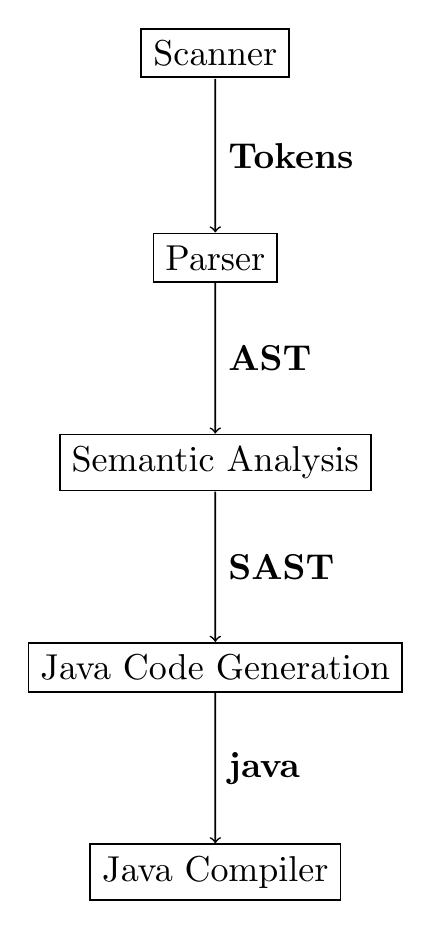
\begin{tikzpicture}[->,node distance=2 cm,
                semithick, scale = 1.3, transform shape]
        \node [draw, rectangle, thick]  (scanner) {Scanner};
        \node [draw, rectangle, below of = scanner] (parser) {Parser};
        \node [draw, rectangle, below of = parser] (semantic) {Semantic Analysis};
        \node [draw, rectangle, below of = semantic] (javagen) {Java Code Generation};
        \node [draw, rectangle, below of = javagen] (java) {Java Compiler};

%% paths
        \path
		         (scanner) edge node [pos=0.5, right] {$\textbf{Tokens}$}  (parser)
                    (parser) edge node [pos=0.5, right] {$\textbf{AST}$} (semantic) 
                    (semantic) edge node [pos=0.5, right] {$\textbf{SAST}$}  (javagen)
                    (javagen) edge  node [pos=0.5, right] {$\textbf{java}$} (java)
                    ;
\end{tikzpicture}
\\ \\ 
As is shown in the diagram, the FRY compiler is split into 4 sections, the Scanner, Parser, Semantic Analysis and Java Code Generation. 
\subsection{Scanner} 
Scans the input program and produces a tokenized output. The Scanner discards all whitespace and comments and reports an error if any invalid character sequences are encountered, such as an invalid identifier or escape sequence. The scanner was written for \texttt{ocamlyacc}.
\subsection{Parser}
Parses the tokenized output of the scanner and generates an \textbf{AST (Abstract Syntax Tree)} . The parser checks the syntax and catches any syntax errors. The parser does not check type or semantics. The parser was written for \texttt{ocamllex} and the AST was written in \texttt{OCaml}.
\subsection{Semantic Analysis}
The Semantic Analyzer parses the AST and checks the type and semantics of every statement. This produces a \textbf{SAST (Semantically-checked Abstract Syntax Tree)}. Each element in the SAST keeps track of its type for use in the java code generation. Any type mismatches or semantic errors will be reported during this step. The Semantic Analyzer and the SAST were written in \texttt{OCaml}.
\subsection{Java Code Generation}
The Java Code Generator parses the SAST and produces corresponding Java code for each statement. At this point the SAST should be fully syntactically and semantically sound, so there should be no errors produced. The java code generator was written in \texttt{OCaml}.

\section{Test Plan}
\subsection{Example Programs and Generated Code}
\subsubsection{Holiday Calendar Example}
A more detailed description of this example is included in \ref{sec:cal_example}.
\textbf{FRY Source Code}
\begin{lstlisting}
# Checks if the date is valid (i.e. no Feb 30th)
bool isValidDate(str mon, int day){
  if ( day > 28 and mon == "Feb"){
    ret false;
  }
  if ( day == 31 ){
    if ( mon == "Sep" or mon == "Apr" or mon == "Jun" or mon == "Nov"){
      ret false;
    }
    else {
      ret true;
    }
  }
  ret true;
}
# Define our file layout
Layout date = {str: mon, int: day, int: year, str: holiday};

# read in the file with the holiday listing
Table holidays = Table (Layout date);
holidays = Read("holidays.txt",",");

str holiday_name;
Table calendar = Table (Layout date);
str List holiday_list;
Table matching_days;

# Generate a calendar, marking the holidays down
for ( mon <- [ "Jan", "Feb", "Mar", "Apr", "May", "Jun", "Jul", "Aug", "Sep", "Oct", "Nov", "Dec" ]){
  for ( day <- [ 1 to 31 ]) {
    if(isValidDate(mon, day)){
        matching_days = [ i | i <- holidays; i.{mon} == mon and i.{day} == day ];
        holiday_list = Column(matching_days, "holiday");
        holiday_name = holiday_list[0];
        Append(calendar, Layout date {mon, day, 2015,holiday_name});
    }
  }
}

Write("holiday-calendar.txt", calendar);
\end{lstlisting}
\vspace{5mm}
\textbf{Generated Java Code}
\begin{lstlisting}[language=Java,
basicstyle=\ttm,
commentstyle=\color{comment}\ttm,
otherkeywords={},             % Add keywords here
keywordstyle=\ttb\color{deepblue},
stringstyle=\color{deepgreen},
frame=tb,                         % Any extra options here
showstringspaces=false,            
breaklines=true]
import fry.*;
import java.util.Arrays;
import java.io.IOException;
import java.util.ArrayList;

public class fry {
 public static class date extends FRYLayout {
   public String mon;
   public Integer day;
   public Integer year;
   public String holiday;
    public date(String mon, Integer day, Integer year, String holiday) {
      super();
     this.holiday = holiday;
     this.year = year;
     this.day = day;
     this.mon = mon;
   }
    public date() {
     super();
   }
    public String toString() {
     return mon.toString() + "|" + day.toString() + "|"
         + year.toString() + "|" + holiday.toString();
   }
 }
  public static Boolean isValidDate(String mon, Integer day) {
   if (day > 28 && mon.equals("Feb")) {
     return false;
   }
    if (day.equals(31)) {
     if (mon.equals("Sep") || mon.equals("Apr") || mon.equals("Jun")
         || mon.equals("Nov")) {
       return false;
     } else {
       return true;
     }
    }
    return true;
 }
  public static void main(String[] args) throws IOException {
   ;
   FRYTable holidays = new FRYTable(new date());
   holidays.readInput(IOUtils.Read("holidays.txt", ","));
   String holiday_name;
   FRYTable calendar = new FRYTable(new date());
   FRYList<String> holiday_list;
   FRYTable matching_days;
   for (String mon : new ArrayList<String>(Arrays.asList(
  new  String[]{("Jan"), ("Feb"), ("Mar"), 
  ("Apr"), ("May"), ("Jun"), ("Jul"), ("Aug"), 
  ("Sep"), ("Oct"), ("Nov"), ("Dec")}))) {
     {
       for (Integer day : FRYListFactory.getGeneratedFryList(1, 31)) {
         {
           if (isValidDate(mon, day)) {
             FRYList<String[]> __ret_data__ = new FRYList<String[]>(
                 holidays.getData().size());
             for (String[] i : holidays.getData()) {
                if ((((i[holidays.layout.getIdByName("mon")])))
                   .equals(mon)
                   && (new Integer(
                       Integer.parseInt(i[holidays.layout
                           .getIdByName("day")])))
                       .equals(day)) {
                 __ret_data__.add(i);
               }
             }
             FRYTable __tmp_tbl__ = new FRYTable(__ret_data__,
                 holidays.layout);
             ;
             matching_days = __tmp_tbl__;
             ;
             holiday_list = matching_days.getColumn("holiday");
             holiday_name = holiday_list.get(0);
             IOUtils.Append(calendar, new date(mon, day, 2015,
                 holiday_name));
           }
          }
       }
     }
   }
   IOUtils.Write("holiday-calendar.txt", calendar);
 }
}
\end{lstlisting}


\subsubsection{Filtering Example}
A more detailed description of this example is included in \ref{sec:filt_example}.
\textbf{FRY Source Code}
\begin{lstlisting}
# Define source layout and read source data
Layout weblog = {str: date, str: site, str: user};
Table weblog_data = Table (Layout weblog);
weblog_data = Read("website_hits.txt","|");

# Filter required records
Table frodo_facebook = [i | i <- weblog_data; i.{site} == "facebook.com" and i.{user} == "Frodo"];
Table sam_google = [i | i <- weblog_data; i.{site} == "google.com" and i.{user} == "Sam"];

# write out filtered records to respective files
Write("frodo_facebook.txt", frodo_facebook);
Write("sam_google.txt", sam_google);
\end{lstlisting}
\vspace{5 mm}
\textbf{Generated Java Code}
\begin{lstlisting}[language=Java,
basicstyle=\ttm,
commentstyle=\color{comment}\ttm,
otherkeywords={},             % Add keywords here
keywordstyle=\ttb\color{deepblue},
stringstyle=\color{deepgreen},
frame=tb,                         % Any extra options here
showstringspaces=false,            
breaklines=true]
package fry;
import java.util.Arrays;
import java.io.IOException;
import java.util.ArrayList;

public class mainTest {
  public static class weblog extends FRYLayout {
    public String date;
    public String site;
    public String user;

    public weblog(String date, String site, String user) {

      super();
      this.user = user;
      this.site = site;
      this.date = date;
    }

    public weblog() {
      super();
    }
    
    public String toString() {
      return date.toString() + "|" + site.toString() + "|"
          + user.toString();
    }
  }

  public static void main(String[] args) throws IOException {
    ;
    FRYTable weblog_data = new FRYTable(new weblog());
    weblog_data.readInput(IOUtils.Read("website_hits.txt", "|"));
    FRYTable frodo_facebook;
    {
      FRYList<String[]> __ret_data__ = new FRYList<String[]>(weblog_data
          .getData().size());
      for (String[] i : weblog_data.getData()) {

        if ((((i[weblog_data.layout.getIdByName("site")])))
            .equals("facebook.com")
            && (((i[weblog_data.layout.getIdByName("user")])))
                .equals("Frodo")) {
          __ret_data__.add(i);
        }
      }
      FRYTable __tmp_tbl__ = new FRYTable(__ret_data__,
          weblog_data.layout);
      frodo_facebook = __tmp_tbl__;
    }
    FRYTable sam_google;
    {
      FRYList<String[]> __ret_data__ = new FRYList<String[]>(weblog_data
          .getData().size());
      for (String[] i : weblog_data.getData()) {

        if ((((i[weblog_data.layout.getIdByName("site")])))
            .equals("google.com")
            && (((i[weblog_data.layout.getIdByName("user")])))
                .equals("Sam")) {
          __ret_data__.add(i);
        }
      }
      FRYTable __tmp_tbl__ = new FRYTable(__ret_data__,
          weblog_data.layout);
      sam_google = __tmp_tbl__;
    }
    IOUtils.Write("frodo_facebook.txt", frodo_facebook);
    IOUtils.Write("sam_google.txt", sam_google);
  }
}
\end{lstlisting}

\subsection{Test Suite}
All testing performed was functional testing. Every time a new functionality was added to FRY, I added in a few tests to test that functionality. A shell script was written which automated running through these tests. The shell script compiles and executes a specific program, and diffs the output of execution against the expected output. If an error occured in any of the phases (compilation, java compilation, execution), the error would be caught an printed to stdout. The source code for the testing driver script - \textbf{run\_tests.sh} are located here \ref{ref:runtests} - and all of the tests are located here \ref{ref:tests}.

\section{Lessons Learned}

When I first learned we had to create our own programming language and compiler, it sounded impossible. And in fact, working on this project only reinforced that notion. While I managed somehow to come out of this class with a (somewhat) working compiler for FRY, the amount of effort needed to implement even the most basic compiler was fairly surprising. At the least, it put things in perspective and taught me just how much effort has gone into GCC, the Java Compiler, even the Bash interpreter; and how involved these pieces of software really are. The fact that they work so consistently, that they are able to do all of these optimizations, and still compile thousands of source files quickly is a small miracle. 

While I did not get the same experience of people working in teams (which is probably not such a big deal, since I do that at work every day), working on a relatively large scale program on my own definitely taught my a thing or two. I definitely felt as though I needed to rush to complete this compiler. Because of that, from the start I implemented some things in a pretty kludgy fashion, and did plenty of things the quick and dirty way. Unfortunately, that mind set turned out to be somewhat "Penny-wise, Pound-foolish" as I eventually paid for my mostly comment-less spaghetti code. Going back and changing certain things became much more painful than it needed to be. I realized it is worthwhile to write clean, maintainable code, even for a relatively short-term project where I was rushing. Had I done that, I may have been able to do \emph{more} over the semester than I accomplished. Something I really came to appreciate was the automated testing. The amount of bugs I introduced would have wreaked havoc had they not been caught by frequent test cycles. 




\section{Appendix}
All modules were built by Tom DeVoe.
\\\\
{\large \textbf{Makefile}}
\lstinputlisting[language=Make,tabsize=1,basicstyle=\ttm,commentstyle=\color{comment}\ttm,otherkeywords={},
keywordstyle=\ttb\color{deepblue},
stringstyle=\color{deepgreen},
frame=tb,
showstringspaces=false,
breaklines=true]{"C:/Users/tdevoe/Documents/Columbia/FRY-lang/src/Makefile.cpy"}
{\large \textbf{ast.ml}}
\lstinputlisting[language=Caml,tabsize=1,basicstyle=\ttm,commentstyle=\color{comment}\ttm,otherkeywords={},
keywordstyle=\ttb\color{deepblue},
stringstyle=\color{deepgreen},
frame=tb,
showstringspaces=false,
breaklines=true]{"C:/Users/tdevoe/Documents/Columbia/FRY-lang/src/ast.ml"}
{\large \textbf{fry.ml}}
\lstinputlisting[language=Caml,tabsize=1,basicstyle=\ttm,commentstyle=\color{comment}\ttm,otherkeywords={},
keywordstyle=\ttb\color{deepblue},
stringstyle=\color{deepgreen},
frame=tb,
showstringspaces=false,
breaklines=true]{"C:/Users/tdevoe/Documents/Columbia/FRY-lang/src/fry.ml"}
{\large \textbf{javagen.ml}}
\lstinputlisting[language=Caml,tabsize=1,basicstyle=\ttm,commentstyle=\color{comment}\ttm,otherkeywords={},
keywordstyle=\ttb\color{deepblue},
stringstyle=\color{deepgreen},
frame=tb,
showstringspaces=false,
breaklines=true]{"C:/Users/tdevoe/Documents/Columbia/FRY-lang/src/javagen.ml"}
{\large \textbf{parser.mly}}
\lstinputlisting[language=Caml,tabsize=1,basicstyle=\ttm,commentstyle=\color{comment}\ttm,otherkeywords={},
keywordstyle=\ttb\color{deepblue},
stringstyle=\color{deepgreen},
frame=tb,
showstringspaces=false,
breaklines=true]{"C:/Users/tdevoe/Documents/Columbia/FRY-lang/src/parser.mly"}
{\large \textbf{sast.mli}}
\lstinputlisting[language=Caml,tabsize=1,basicstyle=\ttm,commentstyle=\color{comment}\ttm,otherkeywords={},
keywordstyle=\ttb\color{deepblue},
stringstyle=\color{deepgreen},
frame=tb,
showstringspaces=false,
breaklines=true]{"C:/Users/tdevoe/Documents/Columbia/FRY-lang/src/sast.mli"}
{\large \textbf{scanner.mll}}
\lstinputlisting[language=Caml,tabsize=1,basicstyle=\ttm,commentstyle=\color{comment}\ttm,otherkeywords={},
keywordstyle=\ttb\color{deepblue},
stringstyle=\color{deepgreen},
frame=tb,
showstringspaces=false,
breaklines=true]{"C:/Users/tdevoe/Documents/Columbia/FRY-lang/src/scanner.mll"}
{\large \textbf{SemanticAnalysis.ml}}
\lstinputlisting[language=Caml,tabsize=1,basicstyle=\ttm,commentstyle=\color{comment}\ttm,otherkeywords={},
keywordstyle=\ttb\color{deepblue},
stringstyle=\color{deepgreen},
frame=tb,
showstringspaces=false,
breaklines=true]{"C:/Users/tdevoe/Documents/Columbia/FRY-lang/src/SemanticAnalysis.ml"}
{\large \textbf{FRYLayout.java}}
\lstinputlisting[language=Java,tabsize=1,basicstyle=\ttm,commentstyle=\color{comment}\ttm,otherkeywords={},
keywordstyle=\ttb\color{deepblue},
stringstyle=\color{deepgreen},
frame=tb,
showstringspaces=false,
breaklines=true]{"C:/Users/tdevoe/Documents/Columbia/FRY-lang/src/java/fry/fry/FRYLayout.java"}
{\large \textbf{FRYListFactory.java}}
\lstinputlisting[language=Java,tabsize=1,basicstyle=\ttm,commentstyle=\color{comment}\ttm,otherkeywords={},
keywordstyle=\ttb\color{deepblue},
stringstyle=\color{deepgreen},
frame=tb,
showstringspaces=false,
breaklines=true]{"C:/Users/tdevoe/Documents/Columbia/FRY-lang/src/java/fry/fry/FRYListFactory.java"}
{\large \textbf{FRYList.java}}
\lstinputlisting[language=Java,tabsize=1,basicstyle=\ttm,commentstyle=\color{comment}\ttm,otherkeywords={},
keywordstyle=\ttb\color{deepblue},
stringstyle=\color{deepgreen},
frame=tb,
showstringspaces=false,
breaklines=true]{"C:/Users/tdevoe/Documents/Columbia/FRY-lang/src/java/fry/fry/FRYList.java"}
{\large \textbf{FRYTable.java}}
\lstinputlisting[language=Java,tabsize=1,basicstyle=\ttm,commentstyle=\color{comment}\ttm,otherkeywords={},
keywordstyle=\ttb\color{deepblue},
stringstyle=\color{deepgreen},
frame=tb,
showstringspaces=false,
breaklines=true]{"C:/Users/tdevoe/Documents/Columbia/FRY-lang/src/java/fry/fry/FRYTable.java"}
{\large \textbf{InputFile.java}}
\lstinputlisting[language=Java,tabsize=1,basicstyle=\ttm,commentstyle=\color{comment}\ttm,otherkeywords={},
keywordstyle=\ttb\color{deepblue},
stringstyle=\color{deepgreen},
frame=tb,
showstringspaces=false,
breaklines=true]{"C:/Users/tdevoe/Documents/Columbia/FRY-lang/src/java/fry/fry/InputFile.java"}
{\large \textbf{IOUtils.java}}
\lstinputlisting[language=Java,tabsize=1,basicstyle=\ttm,commentstyle=\color{comment}\ttm,otherkeywords={},
keywordstyle=\ttb\color{deepblue},
stringstyle=\color{deepgreen},
frame=tb,
showstringspaces=false,
breaklines=true]{"C:/Users/tdevoe/Documents/Columbia/FRY-lang/src/java/fry/fry/IOUtils.java"}
{\large \textbf{run\_fry.sh}}
\lstinputlisting[language=bash,tabsize=1,basicstyle=\ttm,commentstyle=\color{comment}\ttm,otherkeywords={},
keywordstyle=\ttb\color{deepblue},
stringstyle=\color{deepgreen},
frame=tb,
showstringspaces=false,
breaklines=true]{"C:/Users/tdevoe/Documents/Columbia/FRY-lang/src/run_fry.sh"}
{\large \textbf{compile\_fry.sh}}
\lstinputlisting[language=bash,tabsize=1,basicstyle=\ttm,commentstyle=\color{comment}\ttm,otherkeywords={},
keywordstyle=\ttb\color{deepblue},
stringstyle=\color{deepgreen},
frame=tb,
showstringspaces=false,
breaklines=true]{"C:/Users/tdevoe/Documents/Columbia/FRY-lang/src/compile_fry.sh"}
\label{ref:runtests}
{\large \textbf{run\_tests.sh}}
\lstinputlisting[language=bash,tabsize=1,basicstyle=\ttm,commentstyle=\color{comment}\ttm,otherkeywords={},
keywordstyle=\ttb\color{deepblue},
stringstyle=\color{deepgreen},
frame=tb,
showstringspaces=false,
breaklines=true]{"C:/Users/tdevoe/Documents/Columbia/FRY-lang/utils/run_tests.sh"}
\label{ref:tests}
{\large \textbf{arith\_test01.fry}}
\lstinputlisting{"C:/Users/tdevoe/Documents/Columbia/FRY-lang/testing/arith_test01.fry"}
{\large \textbf{arith\_test01.out}}
\lstinputlisting{"C:/Users/tdevoe/Documents/Columbia/FRY-lang/testing/arith_test01.out"}
{\large \textbf{cond\_test01.fry}}
\lstinputlisting{"C:/Users/tdevoe/Documents/Columbia/FRY-lang/testing/cond_test01.fry"}
{\large \textbf{cond\_test01.out}}
\lstinputlisting{"C:/Users/tdevoe/Documents/Columbia/FRY-lang/testing/cond_test01.out"}
{\large \textbf{cond\_test02.fry}}
\lstinputlisting{"C:/Users/tdevoe/Documents/Columbia/FRY-lang/testing/cond_test02.fry"}
{\large \textbf{cond\_test02.out}}
\lstinputlisting{"C:/Users/tdevoe/Documents/Columbia/FRY-lang/testing/cond_test02.out"}
{\large \textbf{func\_test01.fry}}
\lstinputlisting{"C:/Users/tdevoe/Documents/Columbia/FRY-lang/testing/func_test01.fry"}
{\large \textbf{func\_test01.out}}
\lstinputlisting{"C:/Users/tdevoe/Documents/Columbia/FRY-lang/testing/func_test01.out"}
{\large \textbf{func\_test02.fry}}
\lstinputlisting{"C:/Users/tdevoe/Documents/Columbia/FRY-lang/testing/func_test02.fry"}
{\large \textbf{func\_test02.out}}
\lstinputlisting{"C:/Users/tdevoe/Documents/Columbia/FRY-lang/testing/func_test02.out"}
{\large \textbf{func\_test03.fry}}
\lstinputlisting{"C:/Users/tdevoe/Documents/Columbia/FRY-lang/testing/func_test03.fry"}
{\large \textbf{func\_test03.out}}
\lstinputlisting{"C:/Users/tdevoe/Documents/Columbia/FRY-lang/testing/func_test03.out"}
{\large \textbf{func\_test04.fry}}
\lstinputlisting{"C:/Users/tdevoe/Documents/Columbia/FRY-lang/testing/func_test04.fry"}
{\large \textbf{func\_test04.out}}
\lstinputlisting{"C:/Users/tdevoe/Documents/Columbia/FRY-lang/testing/func_test04.out"}
{\large \textbf{layout\_test01.fry}}
\lstinputlisting{"C:/Users/tdevoe/Documents/Columbia/FRY-lang/testing/layout_test01.fry"}
{\large \textbf{layout\_test01.out}}
\lstinputlisting{"C:/Users/tdevoe/Documents/Columbia/FRY-lang/testing/layout_test01.out"}
{\large \textbf{layout\_test02.fry}}
\lstinputlisting{"C:/Users/tdevoe/Documents/Columbia/FRY-lang/testing/layout_test02.fry"}
{\large \textbf{layout\_test02.out}}
\lstinputlisting{"C:/Users/tdevoe/Documents/Columbia/FRY-lang/testing/layout_test02.out"}
{\large \textbf{layout\_test03.fry}}
\lstinputlisting{"C:/Users/tdevoe/Documents/Columbia/FRY-lang/testing/layout_test03.fry"}
{\large \textbf{layout\_test03.out}}
\lstinputlisting{"C:/Users/tdevoe/Documents/Columbia/FRY-lang/testing/layout_test03.out"}
{\large \textbf{list\_test01.fry}}
\lstinputlisting{"C:/Users/tdevoe/Documents/Columbia/FRY-lang/testing/list_test01.fry"}
{\large \textbf{list\_test01.out}}
\lstinputlisting{"C:/Users/tdevoe/Documents/Columbia/FRY-lang/testing/list_test01.out"}
{\large \textbf{list\_test02.fry}}
\lstinputlisting{"C:/Users/tdevoe/Documents/Columbia/FRY-lang/testing/list_test02.fry"}
{\large \textbf{list\_test02.out}}
\lstinputlisting{"C:/Users/tdevoe/Documents/Columbia/FRY-lang/testing/list_test02.out"}
{\large \textbf{loop\_test01.fry}}
\lstinputlisting{"C:/Users/tdevoe/Documents/Columbia/FRY-lang/testing/loop_test01.fry"}
{\large \textbf{loop\_test01.out}}
\lstinputlisting{"C:/Users/tdevoe/Documents/Columbia/FRY-lang/testing/loop_test01.out"}
{\large \textbf{loop\_test02.fry}}
\lstinputlisting{"C:/Users/tdevoe/Documents/Columbia/FRY-lang/testing/loop_test02.fry"}
{\large \textbf{loop\_test02.out}}
\lstinputlisting{"C:/Users/tdevoe/Documents/Columbia/FRY-lang/testing/loop_test02.out"}
{\large \textbf{loop\_test03.fry}}
\lstinputlisting{"C:/Users/tdevoe/Documents/Columbia/FRY-lang/testing/loop_test03.fry"}
{\large \textbf{loop\_test03.out}}
\lstinputlisting{"C:/Users/tdevoe/Documents/Columbia/FRY-lang/testing/loop_test03.out"}
{\large \textbf{loop\_test04.fry}}
\lstinputlisting{"C:/Users/tdevoe/Documents/Columbia/FRY-lang/testing/loop_test04.fry"}
{\large \textbf{loop\_test04.out}}
\lstinputlisting{"C:/Users/tdevoe/Documents/Columbia/FRY-lang/testing/loop_test04.out"}
{\large \textbf{loop\_test05.fry}}
\lstinputlisting{"C:/Users/tdevoe/Documents/Columbia/FRY-lang/testing/loop_test05.fry"}
{\large \textbf{loop\_test05.out}}
\lstinputlisting{"C:/Users/tdevoe/Documents/Columbia/FRY-lang/testing/loop_test05.out"}
{\large \textbf{table\_test01.fry}}
\lstinputlisting{"C:/Users/tdevoe/Documents/Columbia/FRY-lang/testing/table_test01.fry"}
{\large \textbf{table\_test01.in}}
\lstinputlisting{"C:/Users/tdevoe/Documents/Columbia/FRY-lang/testing/table_test01.in"}
{\large \textbf{table\_test01.out}}
\lstinputlisting{"C:/Users/tdevoe/Documents/Columbia/FRY-lang/testing/table_test01.out"}
{\large \textbf{table\_test02.fry}}
\lstinputlisting{"C:/Users/tdevoe/Documents/Columbia/FRY-lang/testing/table_test02.fry"}
{\large \textbf{table\_test02.in}}
\lstinputlisting{"C:/Users/tdevoe/Documents/Columbia/FRY-lang/testing/table_test02.in"}
{\large \textbf{table\_test02.out}}
\lstinputlisting{"C:/Users/tdevoe/Documents/Columbia/FRY-lang/testing/table_test02.out"}
{\large \textbf{table\_test03.fry}}
\lstinputlisting{"C:/Users/tdevoe/Documents/Columbia/FRY-lang/testing/table_test03.fry"}
{\large \textbf{table\_test03.out}}
\lstinputlisting{"C:/Users/tdevoe/Documents/Columbia/FRY-lang/testing/table_test03.out"}

\end{document}